\documentclass[11pt]{article}
\usepackage{verbatim}
\usepackage{listings}
\usepackage{graphicx}
\usepackage{a4wide}
\usepackage{color}
\usepackage{amsmath}
\usepackage{amssymb}
\usepackage[dvips]{epsfig}
\usepackage[T1]{fontenc}
\usepackage{cite} % [2,3,4] --> [2--4]
\usepackage{shadow}
\usepackage{hyperref}
\usepackage{physics}
\usepackage{url}
\usepackage{tikz}
\usepackage{subcaption}
\usepackage[utf8]{inputenc}




\usetikzlibrary{arrows, shapes}

\setcounter{tocdepth}{2}

\lstset{language=c++}
\lstset{alsolanguage=[90]Fortran}
\lstset{basicstyle=\small}
\lstset{backgroundcolor=\color{white}}
\lstset{frame=single}
\lstset{stringstyle=\ttfamily}
\lstset{keywordstyle=\color{red}\bfseries}
\lstset{commentstyle=\itshape\color{blue}}
\lstset{showspaces=false}
\lstset{showstringspaces=false}
\lstset{showtabs=false}
\lstset{breaklines}

\title{ Computational Physics II \\ FYS-4411 }
\author{Gullik Vetvik Killie\\
		Håkon S.B. Mørk\\
		Jose Emeilio Ruiz Navarro
		}

\begin{document}

\maketitle

\abstract{Fill in abstract}

\section{Introduction}

\section{Methods}
	\subsection{Monte Carlo of the Helium Atom}
		In a quantum mechanical system the energy is given by the expectation value of the Hamiltonian, let \(\Psi_T\) be a proposal for a wavefunction that can describe the system.

		\begin{align}
			E[\hat{H}] = \expval{\hat{H}}{\Psi_T} = \frac{\int{d\vb{R} \Psi_T^*(\vb{R})\hat{H} \Psi_T(\vb{R})  }}{ \int{d\vb{R} \Psi_T^*(\vb{R}) \Psi_T(\vb{R}) }}
		\end{align}

		Let us introduce a local energy: 

		\begin{align}
			E_L(\hat{H}) &= \frac{1}{ \Psi_T(\vb{R}) } \hat{H} \Psi_T(\vb{R}))
		\end{align}

		\begin{align}
			E[\hat{H}] &= \frac{\int{d\vb{R} \Psi_T^*(\vb{R}) \Psi_T(\vb{R}) E_L(\vb{R}))  }}{ \int{d\vb{R} \Psi_T^*(\vb{R}) \Psi_T(\vb{R}) }}
			\intertext{Since the denumeraor is a scalar constant after integrating it we can put it inside the integral in the numerator}
			E[\hat{H}] &= \int{d\vb{R} \frac{\Psi_T^*(\vb{R}) \Psi_T(\vb{R})  }{\int{d\vb{R'} \Psi_T^*(\vb{R'}) \Psi_T(\vb{R'})}}  E_L(\vb{R})  }
			\\
			E[\hat{H}] &= \int{d\vb{R} P(\vb{R}) E_L(\vb{R}) }
		\end{align}

			This probability function with \(P(\vb{R})\) as the pdf, and we can use monte carlo integration to solve the integral. 

		\begin{enumerate}
			\item Initialise system. Give particles a random position and decide how many Monte Carlo Cycles to run.
			\item Start Monte Carlo Calculations
				\begin{enumerate}
					\item Propose a move of the particles according to an algorithm, for example \newline \( \vb{R_{new}} = \vb{R_{old}} + \delta * r \), where \(r\) is a random number in \([0,1]\)
					\item Accept or reject move according to \( P(\vb{R_{new}})/ P(\vb{R_{old}}) \ge r \), where r is a new number. Update position values if accepted.
					\item Calculate energy for this cycle.
				\end{enumerate}
		\end{enumerate}

	\subsection{Helium atom}
		The dimensionless hamiltonian for the Helium atom consists of a kinetic energy part and a potential energy part and is given by

		\begin{align}
			\hat{H} &= -\frac{\nabla^2_1}{2} - \frac{\nabla^2_2}{2} - \frac{Z}{r_1} - \frac{Z}{r_2} + \frac{1}{r_{12}}
		\end{align}

		For the energy to be finite the wavefunction must be constructed so the local energy is finite at all points.

		\begin{align}
			E_L(r_i,r_{12}) &= \frac{1}{\Psi_T} \hat{H} \Psi_T
		\end{align}

		If we consider the case where \(r_i \rightarrow 0\) then the \(- \frac{\nabla^2_i}{2} - \frac{Z}{r_i} \) terms of the hamiltonian could cause the energy to blow up, so we need to make sure that those terms stay finite in the limit.

		\begin{align}
			\lim_{r_i\rightarrow 0} {E_L(r_1,r_{12}) } &= \frac{1}{R_i(r_i)} \left( - \frac{1}{2}\pdv[2]{}{x_k} - \frac{Z}{r_i} \right) R_i(r_i) + G(r_i, r_{ij})
			\\
			\lim_{r_i\rightarrow 0} {E_L(r_1,r_{12}) } &= \frac{1}{R_i(r_i)} \left( - \frac{1}{2}\pdv[2]{}{r_k} - \frac{1}{r_i}\pdv{}{r_i}	 -	 \frac{Z}{r_i} \right) R_i(r_i) + G(r_i, r_{ij})
			\intertext{Derivatives of the wavefunction does not diverge since the wavefunction is finite at all points. so the following terms dominate when the particles approach the center.}
			\lim_{r_i\rightarrow 0} {E_L(r_1,r_{12}) } &= \frac{1}{R_i(r_i)} \left( - \frac{1}{r_i}\pdv{}{r_i}	 -	 \frac{Z}{r_i} \right) R_i(r_i)
			\end{align}

		\begin{align}
			 \frac{1}{R_i(r_i)} \pdv{}{r_i} R_i(r_i)	=  -Z  \qquad{ \text{ This gives the solution }}  \qquad R_i(r_i) = A e^{-Z}
		\end{align}




	\subsection{Derivation of local energies}
		The local energy of is dependant on the Hamiltonian and the wavefunction describing the system, the Hamiltonian incorporates both a kinetic energy part given by \( \frac{\nabla_i^2}{2} \) for each particle
		and a potential energy part given by \(\frac{Z}{r_i}\) and \(\frac{1}{r_{ij}}\), where \(Z\) is the charge of the center, \(r_i\) is the distance for electron \(i\) to the atom center and \(r_{ij}\) is the distance between electron \(l\) and \(m\). Then the local energy is given by the following:

		\begin{align}
			E_L &= \sum_{i,i<j}{\frac{1}{ \Psi_T(\vb{r_i} , \vb{r_{ij}}) } \hat{H} \Psi_T(\vb{r_i} , \vb{r_{ij}})}
			\\
			&=	\sum_{i,i<j}\frac{1}{ \Psi_T(\vb{r_i} , \vb{r_{ij}}) } \left( - \frac{\nabla_i^2}{2} -\frac{Z}{r_i}  -  \frac{Z}{r_j} +  \frac{1}{r_{ij} }  \right) \Psi_T(\vb{r_i} , \vb{r_{ij}})
			\\
			&= \sum_{i,i<j}{-\frac{1}{2\Psi_T} \left(\nabla_i^2 \Psi_T  \right)  -\frac{Z}{r_i}  -  \frac{Z}{r_j} +  \frac{1}{r_{ij} }}
		\end{align}

		Let us change derivation variables:

		\begin{align}
			-\frac{1}{2\Psi_T} \left(\nabla_i^2 \Psi_T  \right) &= \sum_{m=1}^{3}{-\frac{1}{2\Psi_T} \left( \pdv[2]{\Psi_T}{x_m} \right)_i}
			\\
			&= \sum_{m=1}^{3}{-\frac{1}{2\Psi_T} \left( \pdv{}{x_m} \left( \pdv{\Psi_T}{r_i}\pdv{r_i}{x_m} \right) \right)_i}
			\intertext{Since \(r_i = \left( x_1^2 + x_2^2 + x_3^2 \right)^{1/2}\) then \( \pdv{r_i}{x_m} = \pdv{\left( x_1^2 + x_2^2 + x_3^2 \right)^{1/2}}{x_m} =\frac{x_m}{r_i} \)}
			&= \sum_{m=1}^{3}{-\frac{1}{2\Psi_T} \left( \pdv{}{x_m} \left( \pdv{\Psi_T}{r_i}\frac{x_m}{r_i} \right) \right)_i}
			\\
			&= \sum_{m=1}^{3}{-\frac{1}{2\Psi_T} \left( \pdv{\Psi_T}{x_m}{r_i}\frac{x_m}{r_i} + \pdv{\Psi_T}{r_i} \pdv{}{x_m} \left(\frac{x_m}{r_i} \right) \right)_i}
			\intertext{ The term \( \pdv{}{x_m} \left(\frac{x_m}{r_i} \right) \) becomes for the different values for \(m\),  \(\pdv{}{x_1}  \left( \frac{x_1}{\left( x_1^2 + x_2^2 + x_3^2 \right)^{1/2}} \right) = \frac{x_2^2 + x_3^2}{r_i^3}\) so all the values for \(m\) term it should sum up to \( \frac{ 2 (x_1^2 + x_2^2 + x_3^2) }{ r_i^3 } \) }
			&= -\frac{1}{2\Psi_T} \left( \pdv[2]{\Psi_T}{r_i}\frac{x_1^2 + x_2^2 + x_3^2}{r^2_i} + \pdv{\Psi_T}{r_i} \frac{ 2 (x_1^2 + x_2^2 + x_3^2) }{ r_i^3 } \right)_i
			\\
			&= -\frac{1}{2\Psi_T} \left( \pdv[2]{\Psi_T}{r_i} + \pdv{\Psi_T}{r_i} \frac{ 2 }{ r_i } \right)
		\end{align}
		Then the local energy becomes:
		\begin{align}
			E_L = \sum_{i,i<j}{  -\frac{1}{2\Psi_T} \left( \pdv[2]{\Psi_T}{r_i} + \pdv{\Psi_T}{r_i} \frac{ 2 }{ r_i } \right)  -\frac{Z}{r_i}  -  \frac{Z}{r_j} +  \frac{1}{r_{ij} }} \label{eq:localEnergy}
		\end{align}


		\subsubsection{Helium: Simple trialfunction}
		The simple version of the trial function is only dependant on one parameter \( \alpha \) and does not take into account interaction between the two electrons, it is of the form 
		\[ \Psi_T (\vb{r_1}, \vb{r_2}) = \exp{ -\alpha (r_1 + r_2) } \]Let us set this trialfunction into the equation for the local energy \eqref{eq:localEnergy}.
		\begin{align}
			E_L &= \sum_{i,i<j}{  -\frac{1}{2\Psi_T} \left( \pdv[2]{e^{-\alpha (r_i + r_j)}}{r_i} + \pdv{e^{-\alpha (r_i + r_j)}}{r_i} \frac{ 2 }{ r_i } \right)  -\frac{Z}{r_i}  -  \frac{Z}{r_j} +  \frac{1}{r_{ij} }} 
			\\
			E_L &= -\frac{1}{2\Psi_T} \sum_{i=1}^2{ \left( \alpha^2 -\alpha \frac{ 2 }{ r_i } \right) \Psi_T  -\frac{Z}{r_i} +  \frac{1}{r_{ij} } }
			\\
			E_L &= -\alpha^2 + (\alpha-Z) \left( \frac{1}{r_1} + \frac{1}{r_2} \right) + \frac{1}{r_{12}} 
		\end{align}




\section{Results and discussion}
	

As a first attempt to solve the ground state energy for the helium
atom we perform Variational Monte Carlo calculation with a brute force
Metropolis sampling. We do this with two trial wave functions
\[
\psi_{T1}({\bf r_{1}},{\bf r_{2}},{\bf r_{12}})=\exp{\left(-\alpha(r_{1}+r_{2})\right)}
\]
and 
\[
\psi_{T2}({\bf r_{1}},{\bf r_{2}},{\bf r_{12}})=\exp{\left(-\alpha(r_{1}+r_{2})\right)}\exp{\left(\frac{r_{12}}{2(1+\beta r_{12})}\right)},
\]
using $\alpha$ and $\beta$ as variational parameters. Energy values
for the simple wave function, $\psi_{T1}$, using only one variational
parameter $\alpha$, are shown in figure \ref{fig01:alpha_Simple}.
We run the Variational Monte Carlo calculation with $10^{7}$ cycles.
As we see in the figures, the energy minimum occurs when we use $\alpha=1.65$.
Using this value for $\alpha$ we get an energy of $-2.8442934$. 

\begin{figure}
\centering 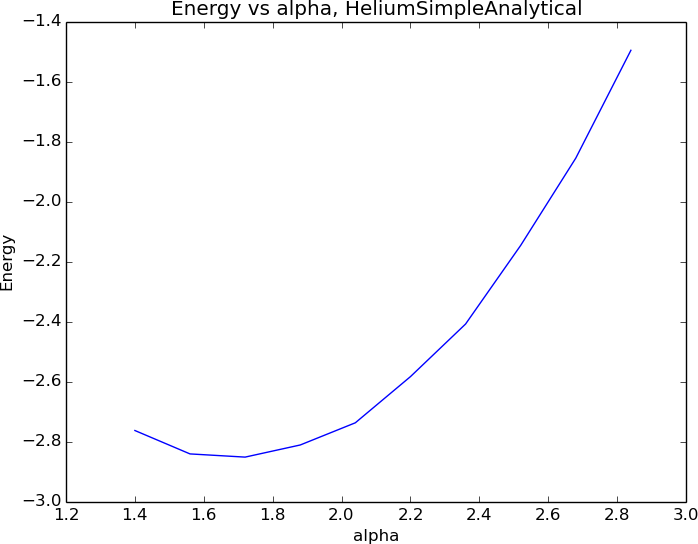
\includegraphics[width=0.45\linewidth]{figures/EnergyVsAlphaHeliumSimpleAnalytical}
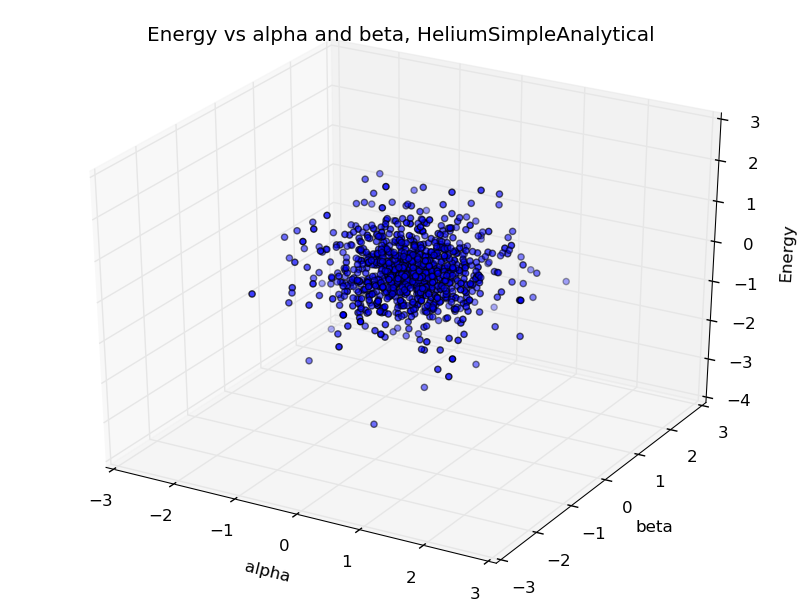
\includegraphics[width=0.45\linewidth]{figures/VarianceVsAlphaHeliumSimpleAnalytical}
\protect\caption{To be filled in}
\label{fig01:alpha_Simple} 
\end{figure}


\begin{figure}
\centering 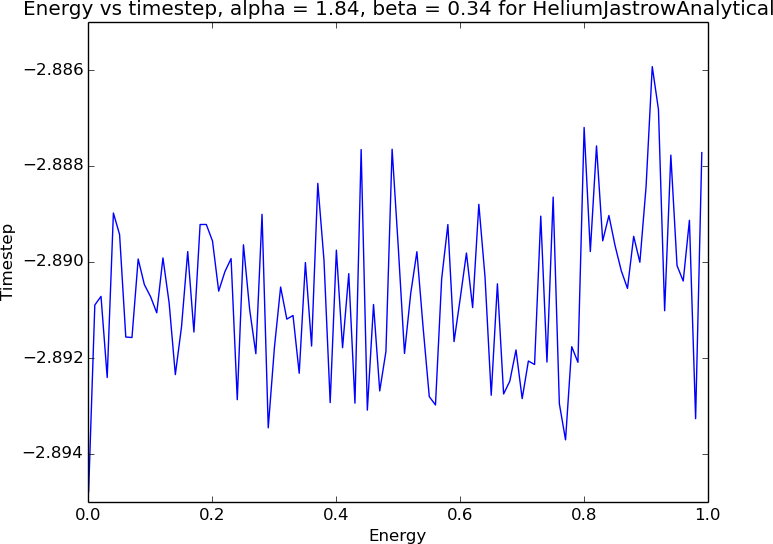
\includegraphics[width=0.45\linewidth]{figures/HeliumJastrowAnalyticalTimeEnergy}
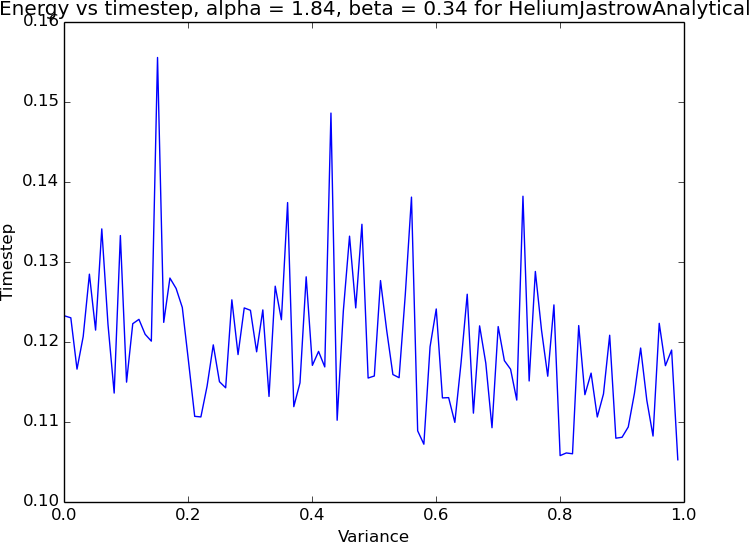
\includegraphics[width=0.45\linewidth]{figures/HeliumJastrowAnalyticalTimeVariance}
\protect\caption{To be filled in}
\label{fig02:timestep} 
\end{figure}

We now look at our second trial function, $\psi_{T2}$. Running over
different values for the two variables $\alpha$ and $\beta$, again
with $10^{7}$ cycles in the Monte Carlo simulation, we get the results
presented in figure \ref{fig03:AlphaBeta}. From this run we find
that the optimal values are $\alpha=1.8$ and $\beta=1.05$. 

\begin{figure}
\centering 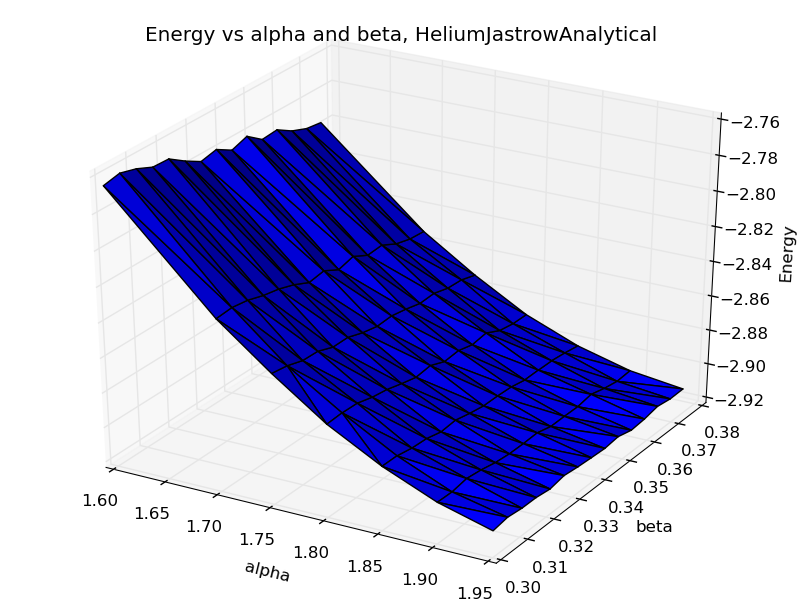
\includegraphics[width=0.45\linewidth]{figures/HeliumJastrowAnalyticalAlphaBetaEnergy}
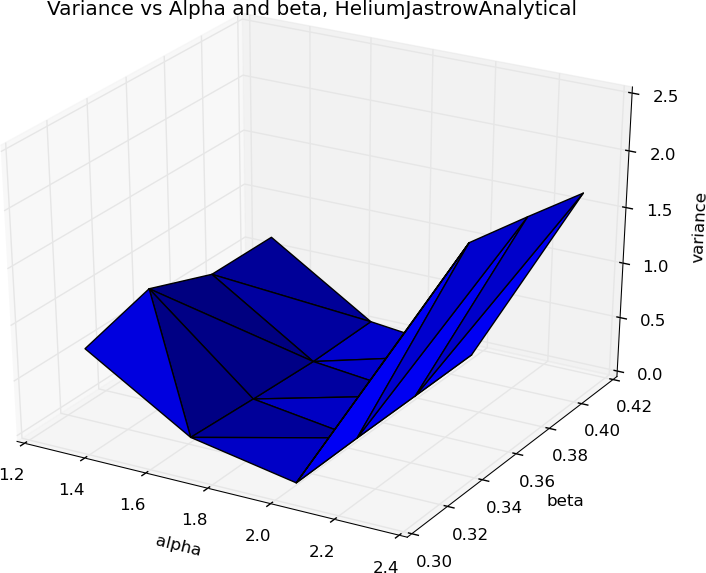
\includegraphics[width=0.45\linewidth]{figures/HeliumJastrowAnalyticalAlphaBetaVariance}
\protect\caption{To be filled in}
\label{fig03:AlphaBeta} 
\end{figure}

\section{Conclusions and perspectives}

\appendix
	
	\section{Testing the VMC}
		\subsection{Hydrogen Atom}
			The wavefunction for the Helium atom can be found exactly and can be used to test our Variational Monte Carlo Calculation since an exact wavefunction should return the exact energy, \( 0.5 \) atomic units with \(0\) variance.

			\[ \Psi(\vb{R}) = r_1 e^{-r_1}  \qquad E_L(r_1) = -\frac{1}{r_1} - \frac{\alpha}{2} \left( \alpha - \frac{2}{r_1} \right) \]

			The unit test a unit named Helium tests the VMC clalculation with a hydrogen wavefunction and returns the correct values.



\end{document}


